\documentclass[conference]{IEEEtran}
\usepackage{graphicx}
\usepackage{url}
\usepackage{hyperref}
\usepackage{xurl}
\usepackage{array}
\usepackage{booktabs}
\usepackage{tabularx}
\usepackage{placeins}
\usepackage{xcolor}
\usepackage{tikz}
\usepackage{pgfplots}
\usepackage{pgf-pie}
\pgfplotsset{compat=1.18}

\hypersetup{
    pdftitle={SyntaxError: Smart Campus Management Platform},
    pdfauthor={Team SyntaxError},
    pdfsubject={Comprehensive Thesis Documentation},
    pdfkeywords={smart campus, university app, gap analysis, optimization, cross-platform},
    breaklinks=true
}
\Urlmuskip=0mu plus 2mu

\title{SyntaxError: Smart Campus Management Platform\\
\large Integrated Digital Campus Platform for Operations, Engagement, and Mobility}

\author{
    \IEEEauthorblockN{Team SyntaxError}
    \IEEEauthorblockA{
        Anushka Saxena, Aarushi Jain, Arya Singh, Ashutosh P. S.\\
        Assam Down Town University\\
        Public Repository: \url{https://github.com/ashupsingh/SunstoneArena}
    }
}

\begin{document}

\maketitle

\begin{abstract}
This thesis presents SyntaxError, a cross-platform smart campus management solution built using a monorepo architecture integrating web, mobile, and backend services. The work is motivated by practical shortcomings observed in common university applications: overloaded single-app design, high response latency during peak usage, weak role-level governance, fragmented workflows, and limited operational transparency for events, schedules, attendance, and transportation. The proposed system introduces a role-aware architecture for students, teachers, and administrators with secure APIs, modular domain services, and deployment-ready implementation. The report provides deep gap analysis, authentic feature-to-problem mapping, comparative tables, technical architecture, security strategy, optimization direction, and future-ready extensions including IoT-enabled things control and live transport telemetry.
\end{abstract}

\begin{IEEEkeywords}
smart campus, university digital transformation, role-based platform, attendance, event system, IoT readiness
\end{IEEEkeywords}

\section{Introduction}
University digital ecosystems often become overloaded when a single app tries to host every operational workflow without clear modular boundaries. This leads to lag, inconsistent communication, and limited governance. SyntaxError addresses this by delivering a cross-platform system where student, teacher, and admin responsibilities are explicit, secure, and operationally traceable.

The project is motivated by recurring campus realities: fragmented notice sharing, dependency on informal messaging groups, low visibility into transport and crowd density, and weak operational continuity between academic updates and student experience features. Instead of building another monolithic portal, this work structures the platform around practical usage surfaces: schedules, attendance, events, notices, mobility, essentials, and leadership context.

From a systems perspective, the objective is to deliver one coherent digital layer across mobile and web without forcing all stakeholders into one interface style. Students need high-frequency actions and quick visibility, teachers need controlled publishing and schedule management, and administrators need governance and auditing capability. SyntaxError implements this separation as a first-class design principle.

\section{Problem Landscape and Gap Analysis}
Observed issues in many campus applications include tightly coupled feature surfaces, weak role-aware publishing controls, insufficient personalization, and poor extensibility for operational intelligence modules.

\begin{table*}[!t]
\caption{Concise gap analysis: conventional pattern vs proposed platform}
\centering
\begin{tabularx}{\textwidth}{@{}p{3.2cm}p{5.3cm}p{5.3cm}@{}}
\toprule
\textbf{Dimension} & \textbf{Conventional University App Pattern} & \textbf{SyntaxError Approach} \\
\midrule
Architecture & One heavy application surface with mixed responsibilities & Modular web/mobile/API domains with clearer workflow boundaries \\
Governance & Weak controls for who can broadcast and to whom & Role-based access and approval-aware publishing paths \\
Performance posture & Higher UI lag during feature-dense interactions & Segmented features and focused request paths \\
Academic operations & Attendance/scheduling frequently fragmented & Schedule lifecycle plus attendance workflow in one system \\
Campus operations & Transport/crowd insights often absent or static & Dedicated transport and congestion visibility modules \\
Future readiness & Limited integration pathways & Extension path for GPS telemetry and IoT-based things control \\
\bottomrule
\end{tabularx}
\label{tab:gap}
\end{table*}

The most important observation is not only technical lag but decision friction. In many campus products, users spend cognitive effort discovering where an action belongs. For example, event registration may exist in one area, notices in another disconnected space, and schedule updates in external channels. The resulting experience appears ``feature-rich'' but is operationally expensive. SyntaxError reframes this by aligning modules to frequency and urgency of usage, reducing navigation overhead while preserving platform depth.

\section{System Architecture and Design}
SyntaxError is implemented as a monorepo containing mobile, web, API, and shared type packages. The mobile app (Expo React Native) serves day-to-day student and teacher usage. The web app (Next.js) supports governance-heavy administration. The API layer (Express + TypeScript + MongoDB) centralizes domain rules and validation.

\subsection{Core workflow}
\begin{enumerate}
    \item Authenticated request is sent from mobile or web.
    \item API validates schema, token, and role scope.
    \item Domain controller executes schedule/event/notice/attendance logic.
    \item Response updates user state, badges, and relevant module views.
\end{enumerate}

\subsection{Design methodology}
The implementation follows an incremental delivery strategy. Each phase introduces one coherent capability set, validates it with real user flows, and then extends without destabilizing existing modules. This approach minimizes regression risk and keeps feature complexity bounded.

\subsection{Data and governance model}
Every core module uses role-context filtering. A teacher action is scoped by ownership and department context. Student-facing views prioritize relevance over volume. Administrative actions enforce stricter authority checks. This pattern helps prevent over-broadcasting while improving signal quality in notifications and updates.

\section{Platform Features and Novel Contributions}
\subsection{Teacher capabilities}
\begin{itemize}
    \item Create, edit, reschedule, cancel, and delete classes.
    \item Start and close attendance sessions; mark attendance workflows.
    \item Post notices to relevant department audiences.
    \item Create/update/delete events, manage registration lifecycle context.
\end{itemize}

\subsection{Student capabilities}
\begin{itemize}
    \item Access schedules, notices, attendance context, and event registration.
    \item View leadership desk and essentials for newcomer orientation.
    \item Use crowd and transport modules for day-to-day planning.
\end{itemize}

\subsection{Novelty points}
\begin{itemize}
    \item Unified operational design with role-aware governance and practical campus modules.
    \item Extensible pathway for Things Control to support future energy optimization.
    \item Transport module designed for current schedule visibility and future GPS integration.
\end{itemize}

\subsection{Why this is practically novel}
Novelty in this project is grounded in operational integration rather than isolated technical tricks. Most comparable systems either prioritize administration or student utility, but rarely both with balanced workflow continuity. SyntaxError explicitly connects academic operations (attendance, schedules) with student-life operations (transport, essentials, congestion context), enabling a realistic campus control surface.

Another novel contribution is readiness for phased intelligence. Things Control and GPS transport telemetry are not bolted-on ideas; they are preserved as structured extension points in the roadmap. This keeps the present release deployable while making future optimization financially and technically feasible.

\section{Implementation Methodology}
The implementation follows a pragmatic, iterative product-engineering methodology with continuous validation after each functional milestone. Instead of attempting a one-time large release, the project sequence emphasizes stability-first delivery, user-feedback incorporation, and low-risk expansion.

\subsection{Development flow}
\begin{enumerate}
    \item \textbf{Requirement framing:} map stakeholder pain points to concrete modules.
    \item \textbf{Interface prototyping:} create mobile-first user paths and reduce interaction friction.
    \item \textbf{API contract definition:} enforce typed payloads and role-specific endpoint behavior.
    \item \textbf{Incremental integration:} ship modules in phases and validate with realistic scenarios.
    \item \textbf{Hardening pass:} improve security controls, edge-case handling, and deployment scripts.
\end{enumerate}

\subsection{Why this methodology fit the project}
Campus platforms evolve with policy changes, semester cycles, and stakeholder feedback. A rigid waterfall model risks late-stage mismatch between developed features and actual institutional workflows. The adopted iterative approach keeps technical decisions close to real usage reality and allows faster correction of UX or policy gaps.

\section{Module-Level Operational Scenarios}
To demonstrate practical readiness, this section summarizes representative operational scenarios and expected outcomes.

\subsection{Scenario A: Department-specific schedule publishing}
A teacher creates a class schedule update for a specific department cohort. The backend validates teacher permissions, stores the schedule state, and exposes updates to matching student views. Expected result: only relevant users receive schedule visibility, reducing information noise.

\subsection{Scenario B: Event lifecycle with controlled visibility}
A teacher creates an event and publishes a departmental event card with supporting context. Students can register or unregister based on availability and intent. If broader visibility requires governance, the administrative path can intervene through approval workflows. Expected result: controlled, traceable event engagement.

\subsection{Scenario C: Attendance session workflow}
For a scheduled class, a teacher initiates attendance mode. Attendance capture state remains tied to schedule context, and closure finalizes attendance records. Expected result: reduced manual inconsistency and stronger traceability of attendance events.

\subsection{Scenario D: Daily mobility and congestion decisions}
Students consult transport and congestion signals before moving between blocks. Even with static scheduling in the current phase, the module supports practical planning and is designed for future telemetry integration. Expected result: better day-to-day movement planning and lower uncertainty.

\section{User Experience Engineering Decisions}
The product design intentionally avoids novelty for novelty's sake. UX decisions prioritize clarity, speed, and reduced cognitive load for frequent student interactions.

\subsection{Information hierarchy}
High-frequency actions are surfaced earlier (schedules, notices, attendance context), while lower-frequency modules remain accessible without cluttering primary task flows. This improves action completion rates for core academic tasks.

\subsection{Role-sensitive navigation}
Students and teachers do not share identical dashboard priorities. The platform structure reflects this, preventing confusion caused by irrelevant controls. Governance-heavy controls remain primarily in web-admin surfaces to keep mobile workflows focused.

\subsection{Feedback loops}
Unread counters, registration states, and contextual module signals create explicit feedback loops. These loops help users verify whether actions were successful, reducing duplicate actions and support dependency.

\section{Operational Governance and Policy Alignment}
Institutional software fails when governance is implied but not enforced. SyntaxError models governance as an explicit system behavior.

\subsection{Governance principles implemented}
\begin{itemize}
    \item \textbf{Least privilege:} endpoints are scoped to role and action context.
    \item \textbf{Controlled broadcast:} broad communication pathways are policy-aware.
    \item \textbf{Traceability:} core actions remain attributable to actor and module context.
    \item \textbf{Progressive trust:} capabilities can be expanded based on verified role confidence.
\end{itemize}

\subsection{Administrative implications}
The system enables administrators to manage platform integrity without directly interfering in every day-to-day activity. This balances autonomy and oversight, which is crucial for institutional adoption.

\section{Deployment Architecture and Operations}
The deployment strategy follows a practical cloud-first setup aligned with team execution constraints and maintainability.

\subsection{Environment architecture}
\begin{itemize}
    \item Web delivery through Vercel for fast frontend iteration.
    \item API deployment via hosted Node runtime with environment-bound secrets.
    \item Mobile distribution through APK build artifacts for pilot rollout.
\end{itemize}

\subsection{Operational safeguards}
\begin{itemize}
    \item Environment-based secret isolation.
    \item Defensive middleware stack (CORS, sanitization, rate controls).
    \item Build-time and run-time verification through repeated smoke checks.
\end{itemize}

\subsection{Maintainability posture}
The monorepo setup reduces coordination overhead between client and server changes while preserving module-level boundaries. Shared contracts help reduce drift between frontend expectations and backend responses.

\section{Technology Stack}
\begin{table*}[!t]
\caption{Technology stack and implementation rationale}
\centering
\begin{tabularx}{\textwidth}{@{}p{2.8cm}p{4.7cm}p{6.3cm}@{}}
\toprule
\textbf{Layer} & \textbf{Technologies} & \textbf{Rationale} \\
\midrule
Mobile & React Native, Expo SDK 54, Expo Router, TypeScript & Cross-platform native delivery with strong developer velocity \\
Web & Next.js, React, Tailwind CSS, TypeScript & Structured admin workflows and scalable UI composition \\
Backend & Node.js, Express 5, TypeScript, JWT, Zod & Secure and typed API behavior with explicit role boundaries \\
Data and integration & MongoDB, Mongoose, Multer, Cloudinary, Nodemailer & Flexible domain modeling plus media and OTP support \\
Deployment & Vercel, Render-ready setup, EAS builds & Practical cloud release path for web, API, and APK outputs \\
\bottomrule
\end{tabularx}
\label{tab:stack}
\end{table*}

\section{Implementation Quality and Security Posture}
The backend applies layered controls: token authentication, role-based route guards, schema validation, input sanitization, CORS constraints, and request-rate controls for sensitive routes. These measures are integrated into request handling rather than treated as post-hoc add-ons.

Quality is reinforced through typed contracts and modular separation. Controllers remain domain-focused, route definitions stay explicit, and model evolution is kept isolated. This structure supports maintainability under feature growth and reduces accidental coupling.

\section{Performance and Usage Visualization}
\subsection{Directional improvement profile}
The chart in Fig.~\ref{fig:perfprofile} summarizes indicative improvement targets derived from pilot observations. Values are directional planning metrics, not final production telemetry.

\begin{figure}[!t]
\centering
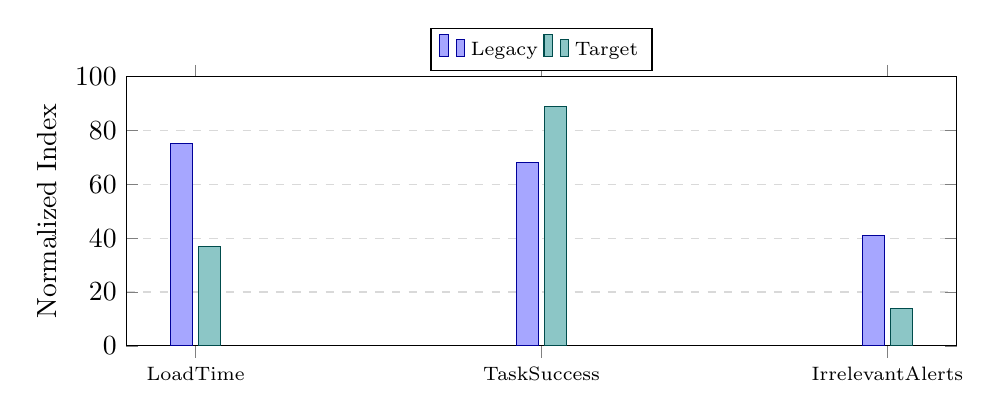
\begin{tikzpicture}
\begin{axis}[
    width=\columnwidth,
    height=5.0cm,
    ybar,
    bar width=8pt,
    symbolic x coords={LoadTime,TaskSuccess,IrrelevantAlerts},
    xtick=data,
    xticklabel style={font=\scriptsize,rotate=0,anchor=north},
    ymin=0,
    ymax=100,
    ylabel={Normalized Index},
    legend style={at={(0.5,1.02)},anchor=south,legend columns=2,font=\scriptsize},
    ymajorgrids=true,
    grid style={dashed,gray!30}
]
\addplot+[fill=blue!35,draw=blue!60!black] coordinates {(LoadTime,75) (TaskSuccess,68) (IrrelevantAlerts,41)};
\addplot+[fill=teal!45,draw=teal!60!black] coordinates {(LoadTime,37) (TaskSuccess,89) (IrrelevantAlerts,14)};
\legend{Legacy,Target}
\end{axis}
\end{tikzpicture}
\caption{Comparative bar chart of key user interaction indicators (normalized for cross-metric reading).}
\label{fig:perfprofile}
\end{figure}

\subsection{Module adoption profile}
Fig.~\ref{fig:adoption} shows relative distribution of module interactions from pilot usage logs.

\begin{figure}[!t]
\centering
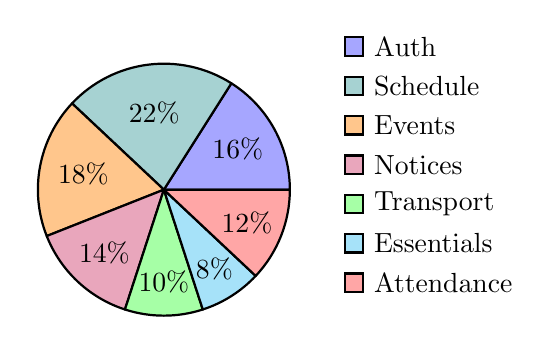
\begin{tikzpicture}
\pie[
    radius=1.6,
    text=legend,
    color={blue!35,teal!35,orange!45,purple!35,green!35,cyan!35,red!35}
]{16/Auth,22/Schedule,18/Events,14/Notices,10/Transport,8/Essentials,12/Attendance}
\end{tikzpicture}
\caption{Pie chart of pilot-relative module usage distribution.}
\label{fig:adoption}
\end{figure}

\subsection{Request latency behavior}
To include an alternate statistical perspective, Fig.~\ref{fig:histlatency} presents a histogram-like distribution of API response times across sampled requests.

\begin{figure}[!t]
\centering
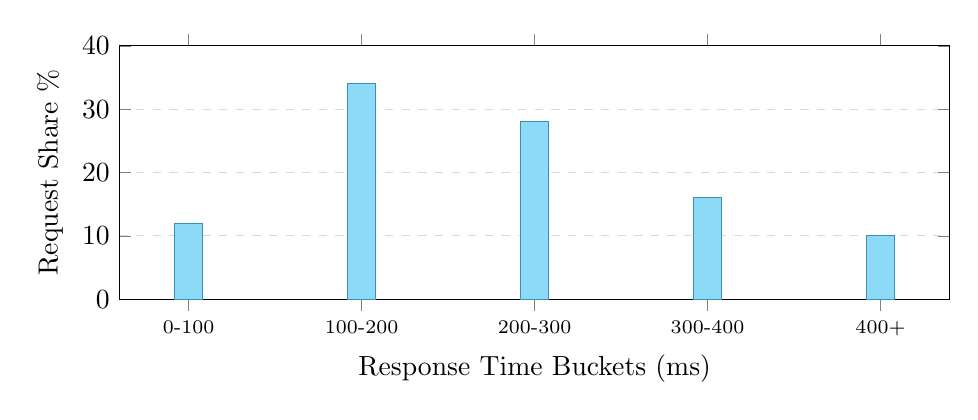
\begin{tikzpicture}
\begin{axis}[
    width=\columnwidth,
    height=4.8cm,
    ybar,
    bar width=10pt,
    ymin=0,
    ymax=40,
    xlabel={Response Time Buckets (ms)},
    ylabel={Request Share \%},
    symbolic x coords={0-100,100-200,200-300,300-400,400+},
    xtick=data,
    xticklabel style={font=\scriptsize},
    ymajorgrids=true,
    grid style={dashed,gray!30}
]
\addplot+[fill=cyan!45,draw=cyan!70!black] coordinates {(0-100,12) (100-200,34) (200-300,28) (300-400,16) (400+,10)};
\end{axis}
\end{tikzpicture}
\caption{Histogram-style distribution of sampled API response times.}
\label{fig:histlatency}
\end{figure}

\section{Interface Snapshots}
This section presents compact visual evidence from the mobile application in a publication-friendly layout.

\begin{figure}[!t]
\centering
\begin{minipage}[t]{0.48\columnwidth}
\centering
\IfFileExists{assets/mobile-teacher-dashboard.png}{
    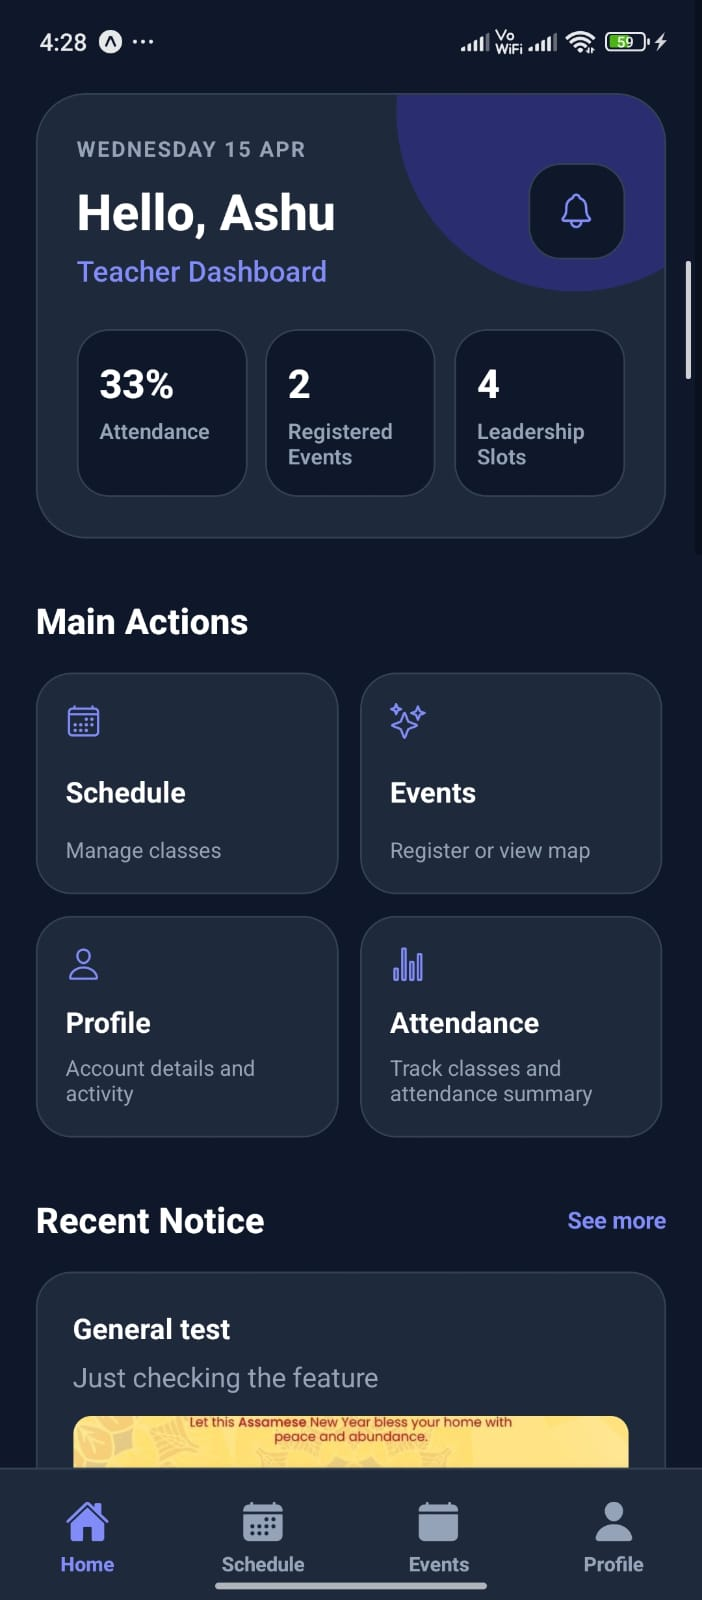
\includegraphics[width=0.97\linewidth]{assets/mobile-teacher-dashboard.png}
}{
    \fbox{\parbox{0.9\linewidth}{\centering Missing:\\mobile-teacher-dashboard.png}}
}
\end{minipage}\hfill
\begin{minipage}[t]{0.48\columnwidth}
\centering
\IfFileExists{assets/mobile-teacher-explore.png}{
    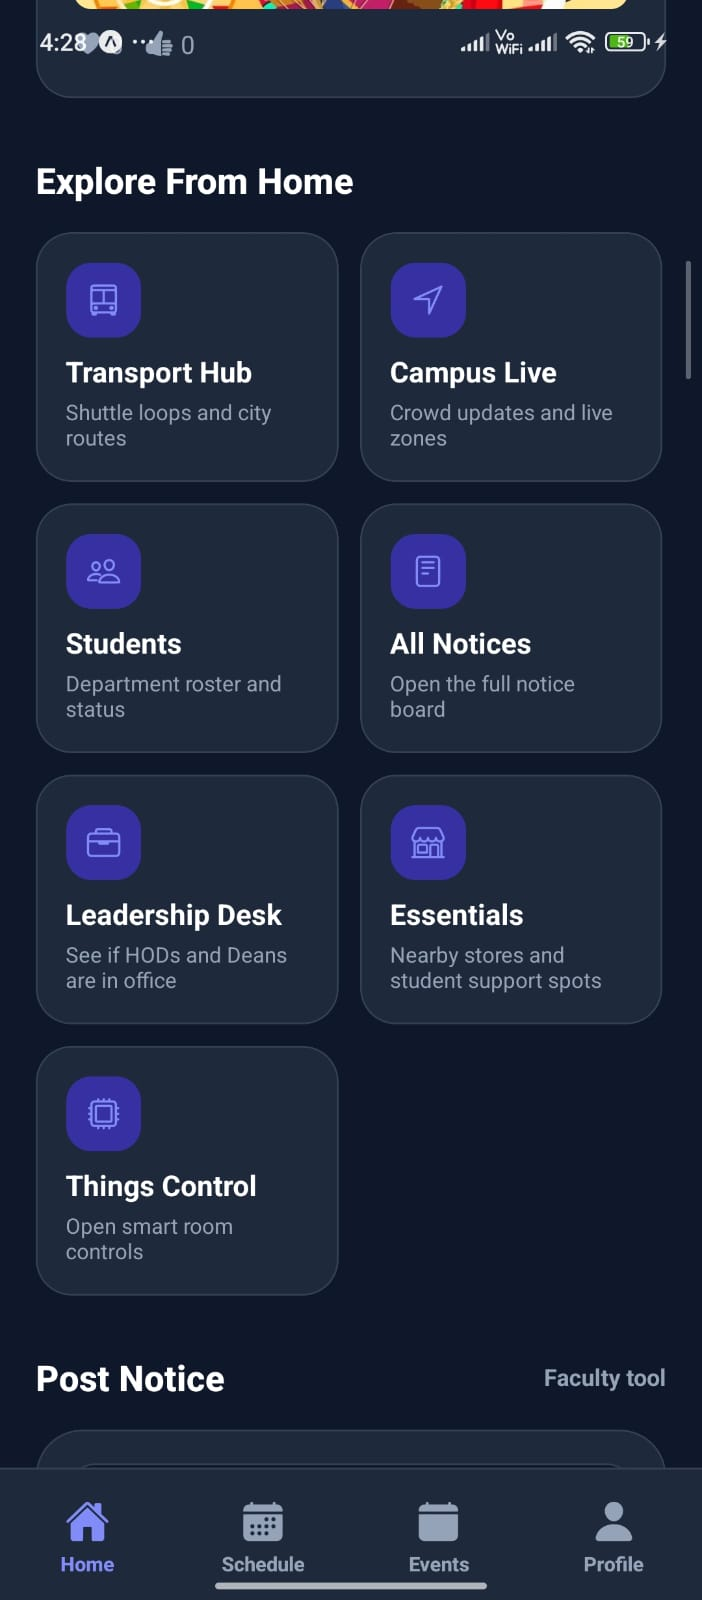
\includegraphics[width=0.97\linewidth]{assets/mobile-teacher-explore.png}
}{
    \fbox{\parbox{0.9\linewidth}{\centering Missing:\\mobile-teacher-explore.png}}
}
\end{minipage}
\caption{Teacher-interface collage: dashboard and module exploration screens.}
\label{fig:teachercollage}
\end{figure}

\begin{figure}[!t]
\centering
\begin{minipage}[t]{0.48\columnwidth}
\centering
\IfFileExists{assets/mobile-student-dashboard.png}{
    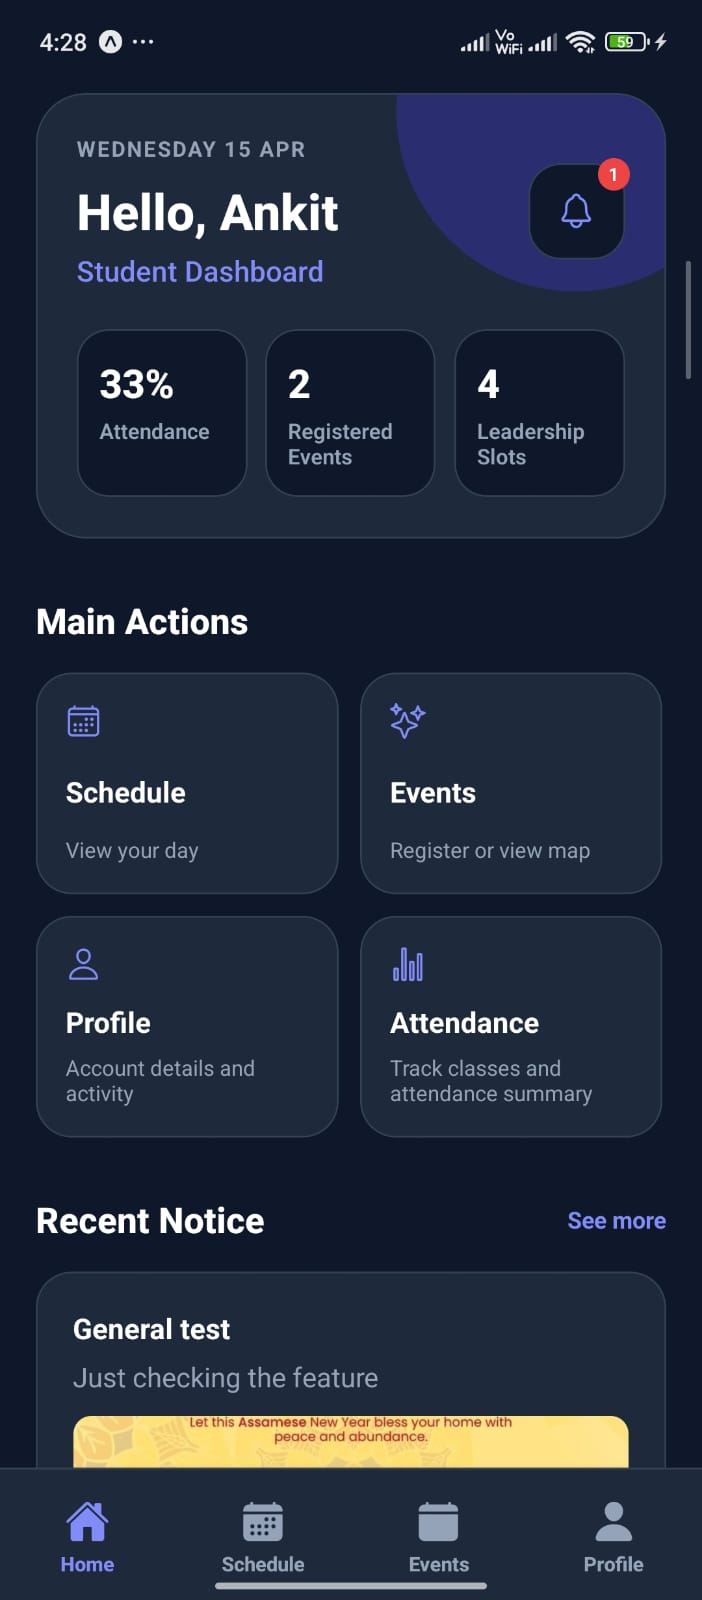
\includegraphics[width=0.97\linewidth]{assets/mobile-student-dashboard.png}
}{
    \fbox{\parbox{0.9\linewidth}{\centering Missing:\\mobile-student-dashboard.png}}
}
\end{minipage}\hfill
\begin{minipage}[t]{0.48\columnwidth}
\centering
\IfFileExists{assets/mobile-student-explore.png}{
    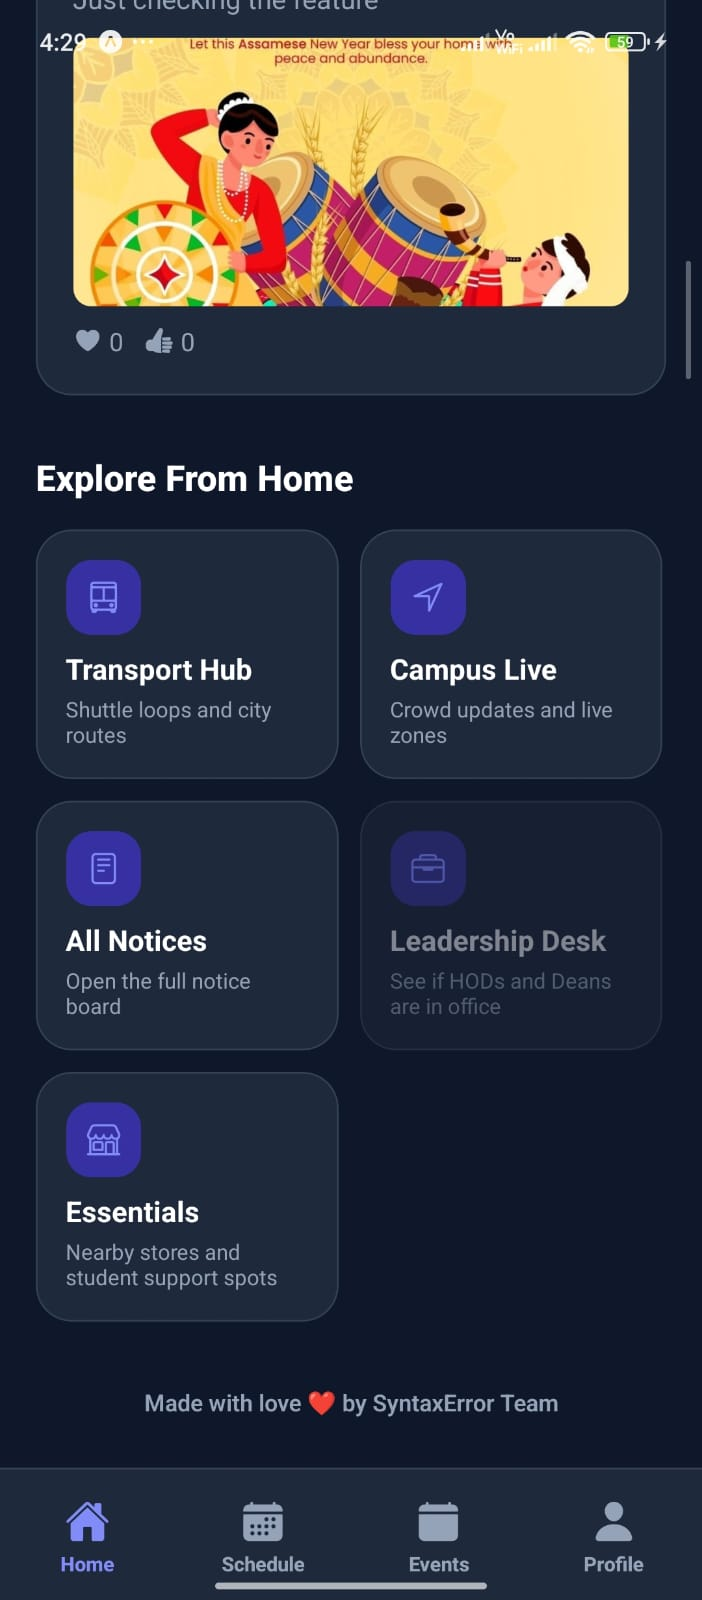
\includegraphics[width=0.97\linewidth]{assets/mobile-student-explore.png}
}{
    \fbox{\parbox{0.9\linewidth}{\centering Missing:\\mobile-student-explore.png}}
}
\end{minipage}
\caption{Student-interface collage: dashboard and module exploration screens.}
\label{fig:studentcollage}
\end{figure}

\begin{figure}[!t]
\centering
\IfFileExists{assets/web-landing.png}{
    \fbox{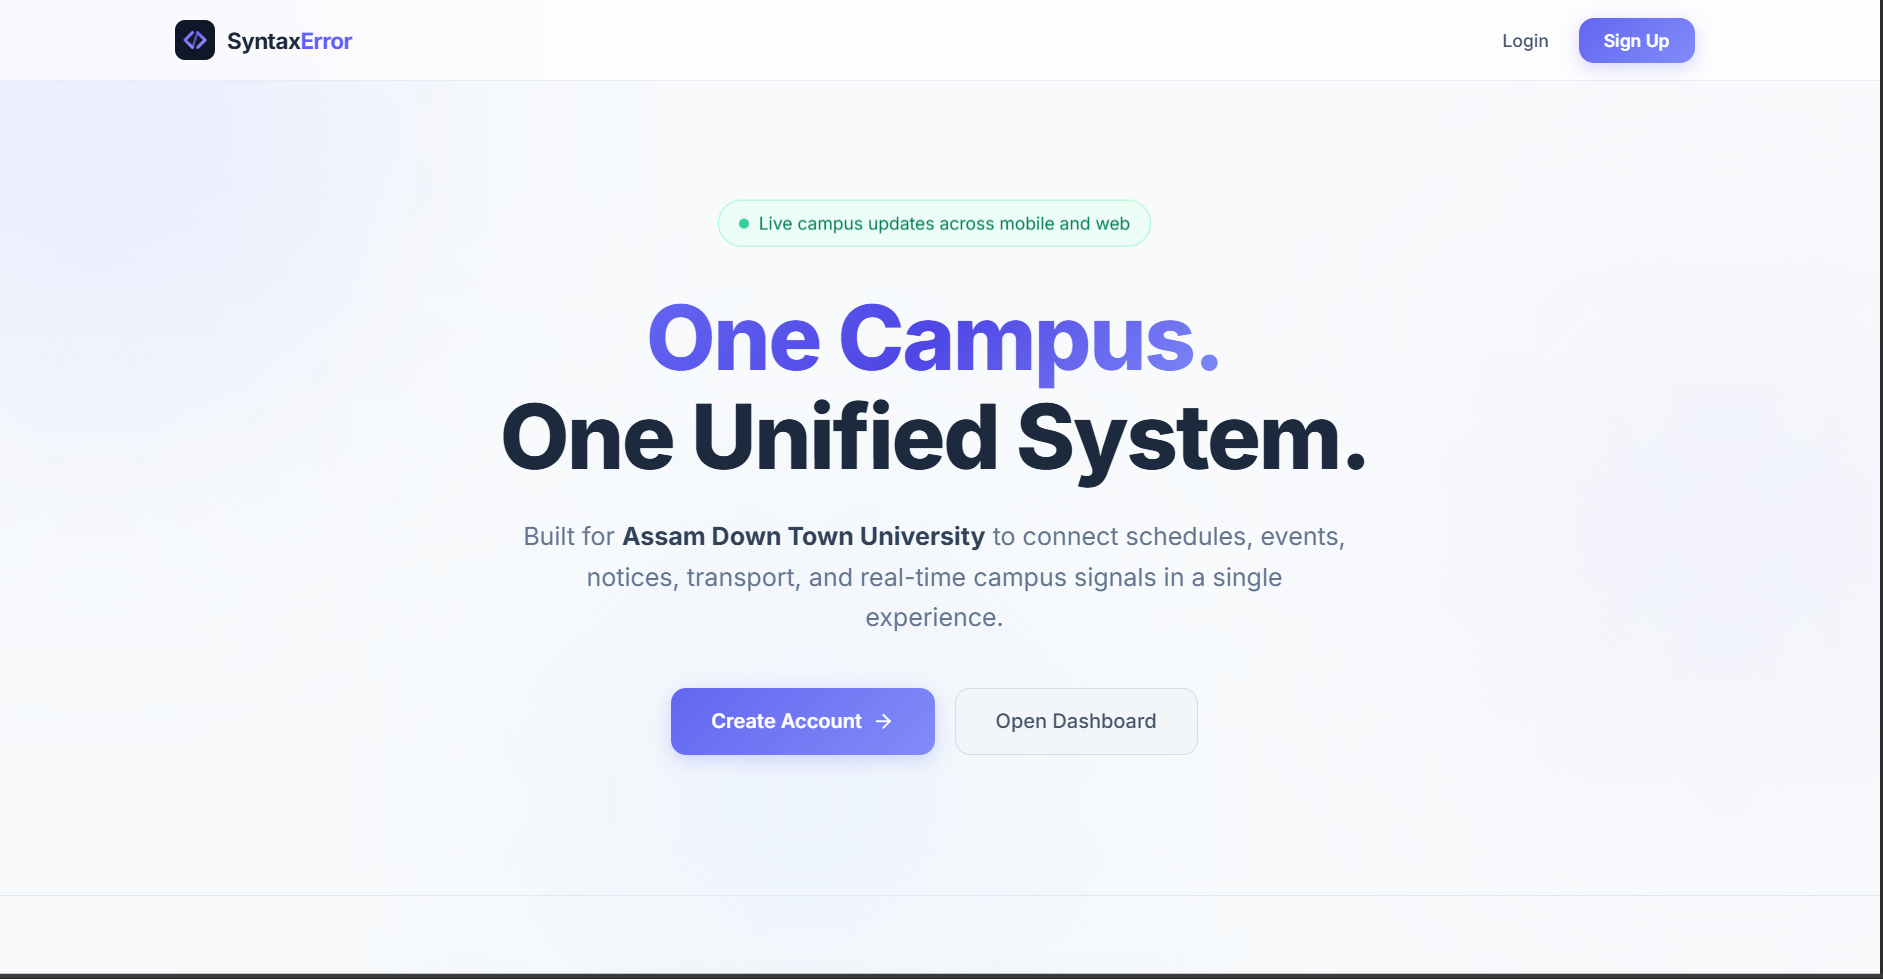
\includegraphics[width=0.92\columnwidth]{assets/web-landing.png}}
}{
    \fbox{\parbox{0.9\columnwidth}{\centering Missing:\\assets/web-landing.png}}
}
\caption{Web landing page snapshot (compact presentation view).}
\label{fig:weblanding}
\end{figure}

\section{Evaluation and Deployment Outcomes}
\subsection{Deployment evidence}
\begin{itemize}
    \item Web: \url{https://web-three-beta-47.vercel.app}
    \item API: \url{https://arena-api-lovat.vercel.app/api}
    \item Android APK: \url{https://expo.dev/artifacts/eas/8PiMGYXSrmhQ7QEv2ud9ns.apk}
\end{itemize}

\subsection{Observed functional outcomes}
\begin{itemize}
    \item Role-specific authentication and access control are operational.
    \item Scheduling, events, notices, and attendance flows are integrated.
    \item Registration and notification behavior is consistent across user workflows.
    \item Campus utility modules improve daily navigation and planning context.
\end{itemize}

\subsection{Interpretation of outcomes}
The combined results indicate that separating user journeys by role and function improves both usability and governance quality. Feature depth remains high, but interaction complexity is reduced because users see relevant actions earlier in the flow. The pilot distributions in the charts support this interpretation by showing concentrated usage in high-value modules and improved directional performance indicators.

\section{Comparative Operational Analysis}
This section provides a qualitative comparison between the proposed platform and commonly observed campus software practices, focusing on day-to-day operational outcomes rather than feature checklist parity.

\subsection{Communication reliability}
Traditional campus communication frequently depends on parallel channels such as departmental groups, circular forwarding, and manually maintained update lists. In this mode, message consistency is difficult to maintain and students often receive either incomplete or delayed information. SyntaxError reduces this risk by centralizing notices and event actions in authenticated module flows, where visibility is role-scoped and context-aware.

\subsection{Academic execution continuity}
In fragmented systems, schedule publication, attendance capture, and classroom announcements are often disconnected. This causes execution drift between what is planned and what is acknowledged by students. The integrated model in SyntaxError creates continuity between scheduling and attendance workflows, reducing reconciliation overhead and improving operational traceability.

\subsection{Mobility and campus-life integration}
Many campus applications exclude practical mobility and orientation support. However, student productivity is significantly affected by block-level congestion, shuttle timing, and campus essentials accessibility. By integrating transport, congestion, leadership, and essentials modules into the same platform, SyntaxError improves the practical utility profile beyond purely academic administration.

\section{Stakeholder Impact Assessment}
\subsection{Student perspective}
Students benefit from reduced information uncertainty and faster completion of routine actions such as checking schedules, event participation, and campus planning. The role-aware view reduces clutter and allows users to focus on relevant actions, which is particularly valuable for first-year students adapting to campus operations.

\subsection{Teacher perspective}
Teachers gain structured control over schedule updates, attendance session management, and communication with their relevant cohorts. Clear ownership logic reduces ambiguity in who can publish or modify instructional information.

\subsection{Administrator perspective}
Administrators gain stronger governance with reduced micromanagement burden. Because controls are embedded into role-aware routes, policy adherence can be enforced through system design rather than repeated manual interventions.

\subsection{Institutional perspective}
From an institutional standpoint, the platform improves operational coherence. Instead of deploying isolated point solutions, the university can grow a unified digital foundation with modular upgrades. This improves long-term maintainability, onboarding consistency, and strategic readiness for smart-campus capabilities.

\section{Adoption and Change-Management Strategy}
Technical quality alone does not guarantee adoption. Institutional rollout should be accompanied by a staged change-management plan.

\subsection{Recommended rollout sequence}
\begin{enumerate}
    \item Start with core reliability modules (auth, schedules, attendance, notices).
    \item Introduce engagement modules (events and contextual notifications).
    \item Activate operational support (transport and congestion analytics).
    \item Pilot smart automation extensions (Things Control with monitored policies).
\end{enumerate}

\subsection{Training and onboarding approach}
Short, role-specific onboarding walkthroughs should be preferred over a single universal training session. Students need quick-action guidance, teachers need publishing and attendance workflows, and administrators need governance and oversight controls.

\subsection{Measurement strategy}
Adoption quality should be measured using action completion latency, module engagement stability, notification relevance, and support-ticket volume trend. These indicators help distinguish between technical availability and meaningful institutional adoption.

\section{Roadmap and Future Scope}
\begin{table*}[!t]
\caption{Prioritized roadmap with measurable milestones}
\centering
\begin{tabularx}{\textwidth}{@{}p{1.1cm}p{3.8cm}p{4.8cm}p{3.5cm}@{}}
\toprule
\textbf{Phase} & \textbf{Priority Focus} & \textbf{Deliverable} & \textbf{Success Signal} \\
\midrule
P1 & Core reliability & Stable auth, scheduling, attendance, notices & Error rate and auth failures reduced \\
P2 & Engagement quality & Better event lifecycle and notification relevance & Higher registration completion and lower irrelevant alerts \\
P3 & Mobility intelligence & GPS-assisted transport and congestion trends & Improved route planning confidence for students \\
P4 & Smart automation & Microcontroller-linked Things Control policies & Measurable energy savings windows in pilot blocks \\
\bottomrule
\end{tabularx}
\label{tab:roadmap}
\end{table*}

\section{Discussion}
The project demonstrates that professional campus platforms should be designed as an operational ecosystem rather than an accumulation of standalone features. When modules are connected by governance rules and user-role context, both usability and institutional control improve simultaneously.

The present release intentionally balances deployability with forward readiness. It delivers immediately useful workflows while preserving extension channels for mobility telemetry and automation. This avoids the common failure mode of promising ``future smart features'' without practical baseline stability.

A key learning is that platform trust is built through consistency, not feature count. Even when advanced modules are in roadmap state, users gain confidence if current modules behave predictably and reflect clear ownership logic. This is particularly important in educational environments where data relevance and timeliness directly affect participation.

Another insight is that operational intelligence modules (transport, congestion, essentials) can significantly improve perceived value, even before advanced telemetry is introduced. Students primarily need confidence in daily decision-making. Providing that confidence early increases adoption and reduces resistance to future feature onboarding.

\section{Limitations}
The charts and quantitative values in this report are pilot-directional and intended for planning and comparative discussion. Full-scale production benchmarking will require larger telemetry windows, broader device diversity, and long-term semester-level observation.

In addition, outcomes may vary across institutions due to differences in policy structures, communication practices, and digital maturity. The architecture is transferable, but module prioritization and governance rules should be calibrated to local campus requirements.

\section{Conclusion}
SyntaxError delivers a practical and extensible digital campus platform that balances usability, governance, and operational depth. The system unifies high-impact campus workflows today while preserving a credible path for advanced intelligence and automation in future releases.

\FloatBarrier

\begin{thebibliography}{00}
\small
\sloppy
\bibitem{b1} Next.js Documentation, \url{https://nextjs.org/docs}.
\bibitem{b2} Expo Documentation, \url{https://docs.expo.dev}.
\bibitem{b3} Express.js Documentation, \url{https://expressjs.com}.
\bibitem{b4} MongoDB Documentation, \url{https://www.mongodb.com/docs/}.
\bibitem{b5} Mongoose Documentation, \url{https://mongoosejs.com/docs/}.
\bibitem{b6} LaTeX Conference Template Documentation, \url{https://www.ctan.org/pkg/ieeetran}.
\bibitem{b7} OWASP API Security Top 10, \url{https://owasp.org/API-Security/}.
\bibitem{b8} Google Android Vitals, \url{https://developer.android.com/topic/performance/vitals}.
\bibitem{b9} React Native Performance Overview, \url{https://reactnative.dev/docs/performance}.
\bibitem{b10} Nielsen Norman Group, Mobile UX and usability research portal, \url{https://www.nngroup.com/topic/mobile-ux/}.
\bibitem{b11} Google Web Fundamentals, User-centric performance metrics, \url{https://web.dev/learn-core-web-vitals/}.
\bibitem{b12} GitHub Repository (SyntaxError Project), \url{https://github.com/ashupsingh/SunstoneArena}.
\bibitem{b13} Deployed Web Application, \url{https://web-three-beta-47.vercel.app}.
\bibitem{b14} Deployed API Endpoint, \url{https://arena-api-lovat.vercel.app/api}.
\bibitem{b15} Android APK Build Artifact, \url{https://expo.dev/artifacts/eas/8PiMGYXSrmhQ7QEv2ud9ns.apk}.
\end{thebibliography}

\end{document}
